\documentclass[11pt,a4paper]{article}
\usepackage[utf8]{inputenc}
\usepackage[T1]{fontenc}
\usepackage[a4paper,margin=2.3cm]{geometry}
\usepackage{graphicx}
\usepackage{caption}
\usepackage{subcaption}
\usepackage{float}
\usepackage{enumitem}

\setlist[itemize]{itemsep=0pt,topsep=2pt}
\captionsetup{labelsep=endash}
\renewcommand{\figurename}{\textsc{Figure}}
\renewcommand{\labelitemi}{---}
\setlength{\parindent}{0pt}

\title{Programmation 3D -- TP3\\[2pt]\large Transformations dépendantes et éclairage de Phong}
\author{Axel Kramer}
\date{}

\begin{document}
\maketitle
\vspace{-2em}

\textit{Les captures ont été faites sous Linux. Le code a été un peu modifié pour tourner aussi sur Mac.}

\section*{Ce qui fonctionne}
\begin{itemize}
  \item Partie 1 : matrice \texttt{model} membre de \texttt{Mesh}, \texttt{updateTransforms()} avec matrice de base, rotations d'Euler, touche \texttt{r} (le second maillage tourne autour du premier).
  \item Partie 2 : maillages colorés par leurs normales (attribut passé du vertex au fragment shader).
  \item Partie 3 : éclairage de Phong (ambiante, diffuse, spéculaire), matrices Model, View et Projection envoyées séparément.
  \item Partie 4 : matériaux de Phong (\texttt{PhongMaterial}), un maillage mat et un maillage brillant de couleurs différentes.
\end{itemize}

\section*{Ce qui n'a pas été fait}
\begin{itemize}
  \item Renommage des attributs du vertex shader en « normales » (indiqué comme pas très important).
\end{itemize}

\section*{1 -- Transformations dépendantes}
\begin{figure}[H]
  \centering
  \begin{subfigure}{0.36\textwidth}
    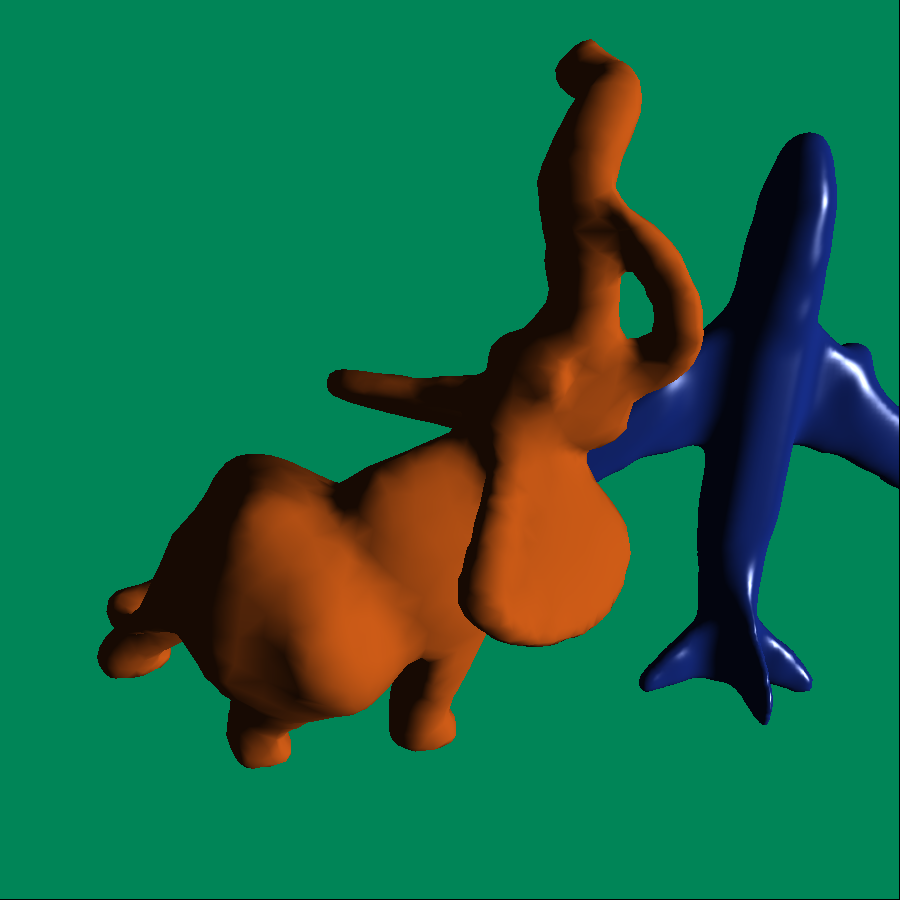
\includegraphics[width=\linewidth]{partie1_initial.png}
    \caption{Position initiale.}
  \end{subfigure}\hspace{0.05\textwidth}
  \begin{subfigure}{0.36\textwidth}
    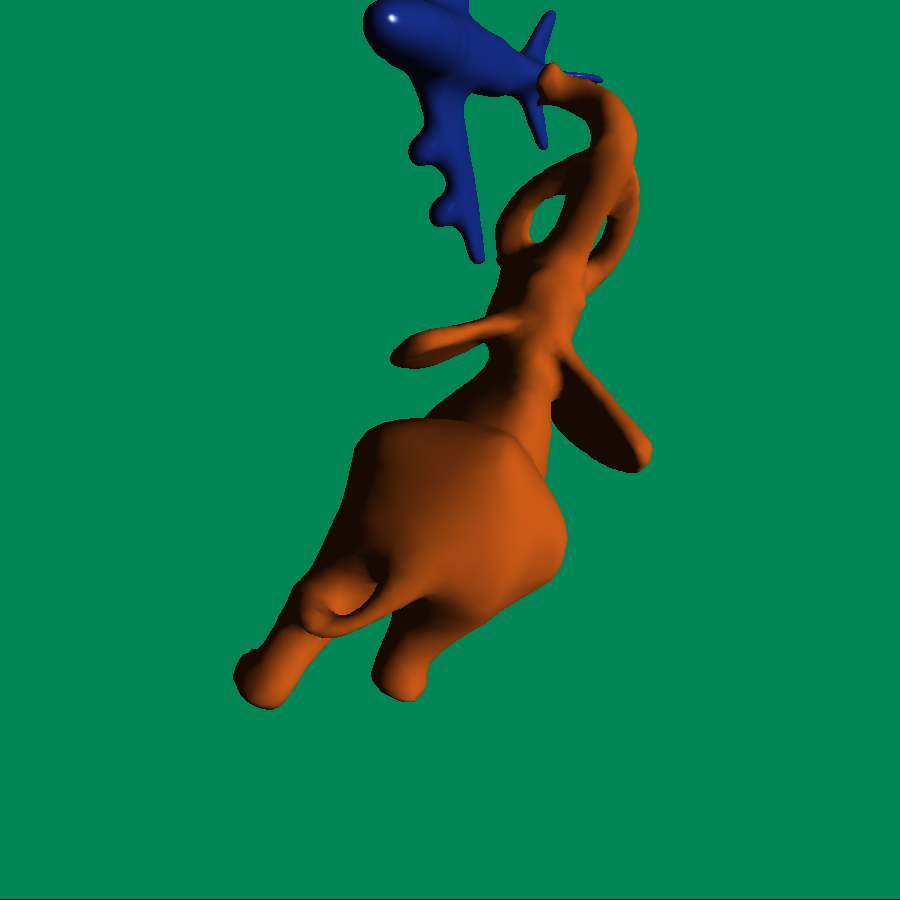
\includegraphics[width=\linewidth]{partie1_rotation.png}
    \caption{Après appui sur \texttt{r}.}
  \end{subfigure}
  \caption{L'éléphant tourne autour du centre (axe $y$), l'avion autour de l'éléphant (axe $z$).}
\end{figure}
Si les maillages tournent sur eux-mêmes, il faut appliquer les rotations avant la translation dans \texttt{updateTransforms()}.

\section*{2 -- Attributs de shaders}
\begin{figure}[H]
  \centering
  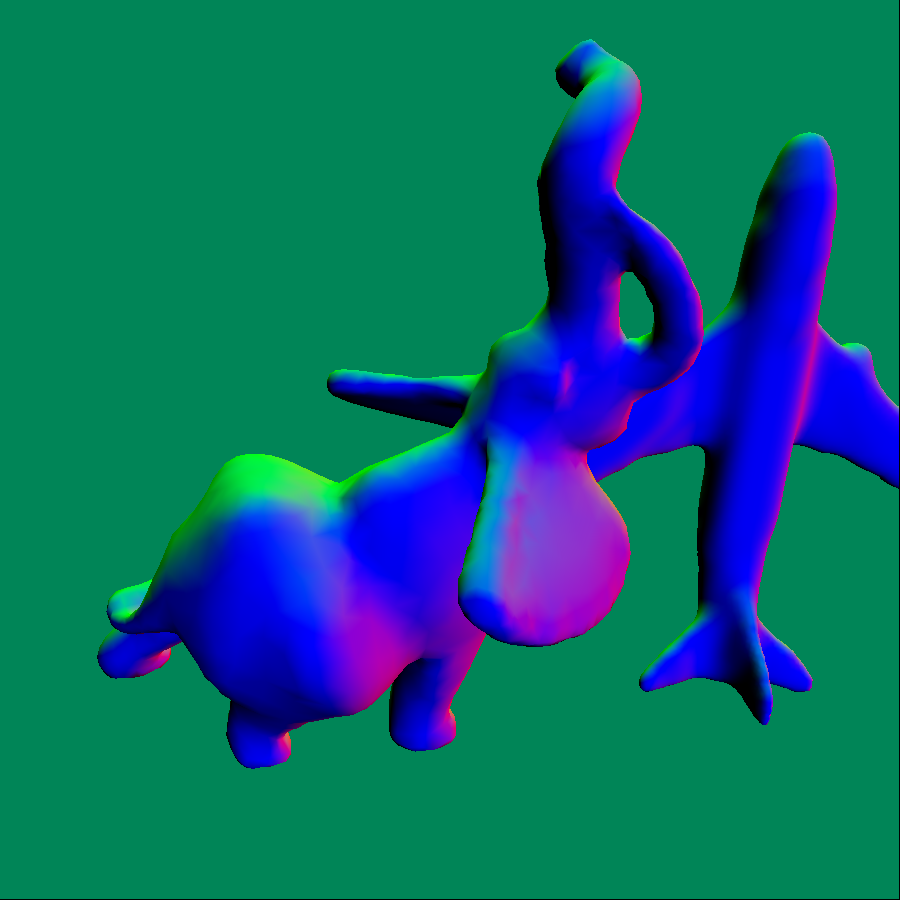
\includegraphics[width=0.42\textwidth]{partie2_normales.png}
  \caption{Maillages colorés par leurs normales.}
\end{figure}

\section*{3 -- Éclairage de Phong}
\begin{figure}[H]
  \centering
  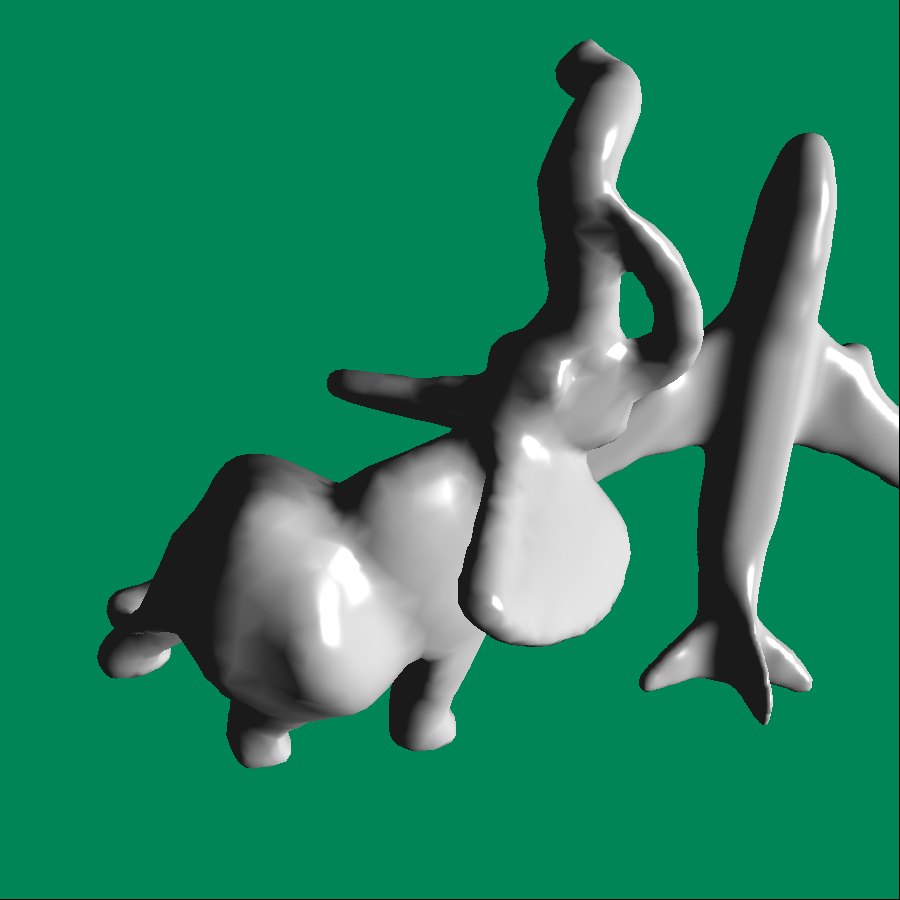
\includegraphics[width=0.42\textwidth]{partie3_phong.png}
  \caption{Éclairage de Phong avec $k_a = k_d = k_s = (1,1,1)$ et une brillance de 32.}
\end{figure}

\section*{4 -- Matériaux de Phong}
\begin{figure}[H]
  \centering
  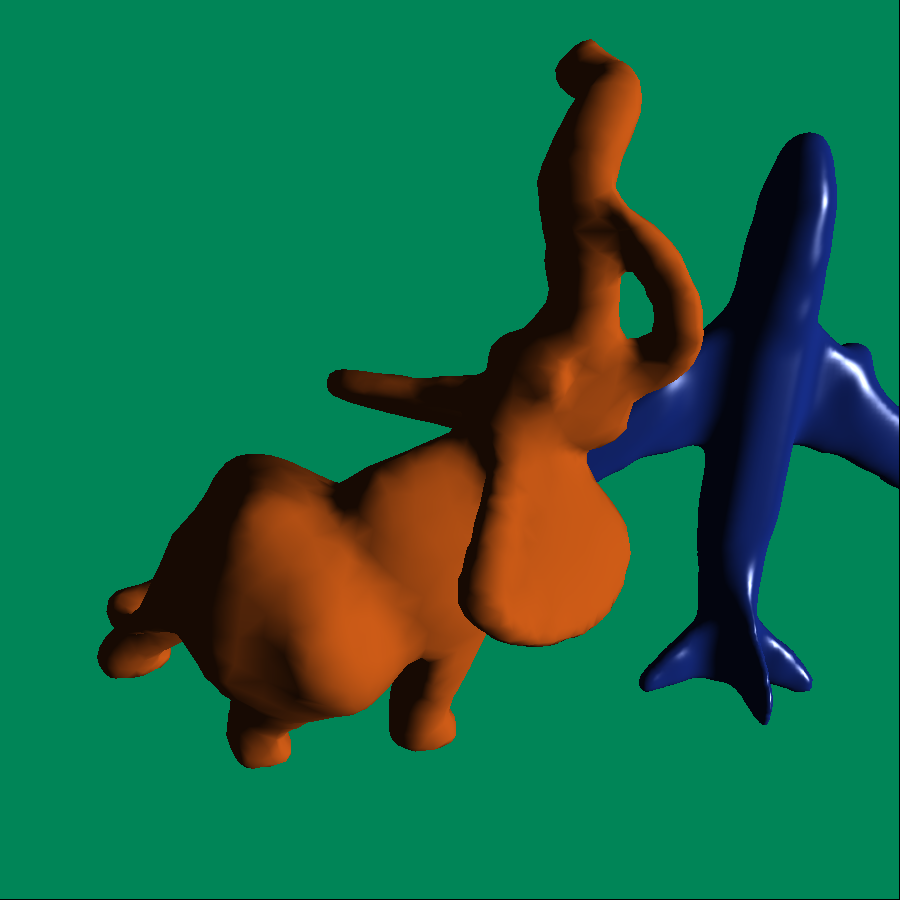
\includegraphics[width=0.42\textwidth]{partie4_materiaux.png}
  \caption{Éléphant très diffus et peu spéculaire (orange, mat), avion peu diffus et très spéculaire (bleu, brillant).}
\end{figure}

\end{document}
